\documentclass[11pt,preprint]{aastex}
\usepackage{amsmath}
\usepackage[top=1in, bottom=1in, left=1in, right=1in]{geometry}
%\usepackage{natbib}
%\usepackage{natbibspacing}
\usepackage{enumitem}
\usepackage{url}
\setlist[itemize]{noitemsep, topsep=0pt}
\setlist[enumerate]{noitemsep, topsep=0pt}
%\setlength{\bibspacing}{0pt}
\setlength{\parskip}{0pt}
\setlength{\parsep}{0pt}
\setlength{\headsep}{6pt}
\setlength{\topskip}{0pt}
\setlength{\topmargin}{0pt}
\setlength{\topsep}{6pt}
\setlength{\partopsep}{0pt}
\setlength{\footnotesep}{8pt}

\begin{document}
\tolerance=10000
\def\simlt{\lower.5ex\hbox{$\; \buildrel < \over \sim \;$}}
\def\simgt{\lower.5ex\hbox{$\; \buildrel > \over \sim \;$}}

\title {LAB 2: Astronomy with the 21-cm Line and Waveguides}

\tableofcontents

\section{Introduction}

\noindent
In this lab, we build upon the signal processing techniques of the previous lab,
applying them to making astronomical measurements with a horn antenna
tuned to frequencies around 1.4 GHz where we can measure 21-cm hyperfine
emission from neutral hydrogen in the Milky Way.  With luck, we should be able
to see evidence of the spiral-arm structure of gas in our galaxy.

In the second half of this lab, we expand our understanding of how signals
propagate through transmission lines to characterize the
cables and reflections in our receiver system, all in service of calibrating
our measurements.

As before, your work should be oriented around producing a high-quality report that
addresses the goals in \S\ref{sec:goals}. From your previous report, you will
be familiar with the need to succintly describe your experimental setup and hardware.
New to this report will be sections describing how you obtained your observations,
the calibration and analysis that went into producing your key results, and the
statistical error in your measurements.

We have a few more suggestions for how to organize your work, building on the 
suggestions of the previous lab:
\begin{itemize}

\item Develop (version-controlled) scripts for taking data from the command line.
Have these scripts save data files with {\bf all the necessary metadata} for
reconstructing your observation. Omitting critical information could
mean you have to redo observations later.

\item Test your reality. How do you know your rotation matrices give you the
right pointing? How do you know if your gain calibration is right? To build
your confidence, you need internal consistency checks, which means deriving
solutions to things you already know the answer to. Find every opportunity
to test things you think you know. It will save you time later.

\item As you conduct observations, think critically about your assumptions and
approximations.  How well have you pointed the horn? How completely did
you cover the aperture for the calibration run? The more you can capture
as you do the work, the more resources you will have for critically analyzing your
results and procedures in your report.

\item By the end, you should have empirical numerical results to report. Remember
that values without errors are meaningless. As you estimate errors, think about how 
well your model matches the data. How can you estimate the
accuracy of your results? Are you confident enough in your analysis to
bet money on your reported accuracy? If not, think about the sources of error
(systematic and otherwise) that may be undermining your confidence.

\end{itemize}


\section{Goals and Instructions for Your Report} \label{sec:goals}

\noindent
As always, lab reports and analysis code must be written {\it individually}. 

The electronic components are such an important part of this
lab that you should include a block diagram of the telescope receiver
in your lab report. You can prepare this either by either hand or
computer. If by hand, you'll have to scan your drawing to get a file you can
insert into your report's tex file. If by computer, you can use your
favorite software for making line drawings.  Although it is dated, {\tt xfig}
comes installed on Linux, so that's an option.

Below is a list of learning goals that your report should demonstrate mastery of.

\begin{itemize}

\item Learn about time. Demonstrate accurate conversion between UTC, PST, LST,
and Julian Day.

\item Learn about telescope pointing and use rotation matrices to convert among spherical
  coordinate systems.

\item Measure a 21-cm line power spectrum from atomic hydrogen in the
  Milky Way at a defined and reproducible location.

\item Calibrate your telescope observations to an absolute scale, remove
systematic instrumental effects in your spectra, and apply noise-reduction
techniques.

\item Learn about Doppler correction and produce spectra with velocities 
calibated relative a standard frame of reference.

\item Fit spectra with Gaussian components to localize celestial structures.

\item Demonstrate undestanding of transmission lines to 
minimize reflections with impedance matching.

\item Derive propagation velocities for radio waves traveling down coaxial cables.

\item Use linear and non-linear least-squares methods to fit models to data and
estimate error.

\end{itemize}

\section{Schedule}

\noindent
This lab covers a lot of new territory, particularly in the realm of data
analysis. Work hard to get good observations early, reserving plenty of
time for analysis and, if necessary, re-observation. A suggested schedule
follows.
\begin{enumerate}

\item {\it Week 1.}
Finish \S\ref{radioastro} and \S \ref{analysis}, and understand \S
  \ref{jultime}. Be prepared to show work, software, and results in class.

\item {\it Week 2.}
Finish \S \ref{meas2}, \S \ref{expt}, and \S \ref{secondweek}. Produce
candidate plots and analysis results for class.

\item {\it Week 3.} Finish any re-observations needed for the first
two weeks, then write your formal
  report. Remember to follow the report guidelines and address the specific
goals in \S\ref{sec:goals}.

\end{enumerate}


\section{What Time Is It?} \label{jultime}

\noindent
From relativity, we know that time depends on
reference frame. Nothing drives this home like sitting on the surface
of an orbiting, spinning sphere.
To deal with this, humans have invented a surfeit of time standards.
We will restrict our attention to those most useful for astronomy.

{\bf Coordinated Universal Time (UTC)} is the Civil Time\footnote{You use
  Civil Time when you set your alarm clock for getting up in the
  morning.} in Greenwich, England, which is 8 hours ahead of 
Pacific Standard Time (PST). In the middle of this course, we switch from
PST to Pacific Daylight Time (PDT); 
${\rm PST}={\rm UTC} - 8$ hr, while ${\rm PDT}={\rm UTC} - 7$ hr). UTC measures
solar time; 24 hours is the time it takes for the Sun to appear
in the same position in the sky on neighboring days.

Another standard, common since the computer era, is {\bf Unix Standard Time}, which measures the
number of seconds since midnight 1 Jan., 1970, UTC. 
This clock is how your computer keeps track of time. All other computer times
are derived from this one; it
is what you get if you call {\tt time.time()}.
You phone/computer uses a quartz crystal oscillator to keep track of 
this time over short intervals.  Over longer intervals, a time-exchange protocol called 
Network Time Protocol (NTP) is used to discipline the on-board clock to 
atomic clocks in timing centers around the world.

{\bf Sidereal Time} is ``star time''; it tells when
distant stars (i.e. not the Sun) rise and set. The sidereal time period is
shorter than the 24-hour Solar time period: $1/356.24$ less, to
be nearly exact. The difference, which corresponds to slightly 
less than 4 minutes per day, comes from how much the Earth's orbit around the
Sun changes the position of the Sun in the sky.
Sidereal time depends on the Earth's spin. The
Earth is constantly slowing owing to tidal friction produced by the
Moon. (Where does the angular momentum go?) The conversion between Civil Time and LST has to be adjusted
periodically by inserting {\it leap seconds}.

{\bf Local Sidereal Time} (LST)
adjusts sidereal time by longitude so that a star of a given {\bf right ascension} 
(RA; the ``longitude" coordinate for celestial sources) transits the local meridian
(the line of longitude that goes right overhead) at the moment
that ${\rm LST}={\rm RA}$. 

The {\bf Julian Day} is a sequential numbering of Solar days since 1 Jan. --4713. 
It
uniquely specifies the date and time (as a fraction of a day) without 
involving 
months (with their nonsensical definitions\footnote{``Thirty days
  hath September\dots''}), leap years, etc. It begins at noon 
in Greenwich. This makes it 12 hours out of phase with UTC, but the
international date line is 12 hours away from UTC, so JD is in sync
with humankind's definition of `when the day begins'. 
On computers, the Julian day is represented as double-precision
float.

The {\bf Modified Julian Day} is a shorter version of Julian Day. MJD is (sigh) 12
hours out of sync with JD, so it is in sync with UTC.
MJD=0 corresponds to 0 hr UT on 17 Nov 1858.

\subsection{ Useful Python Procedures for Time Conversion}

\noindent
Python has several built-in modules for dealing with time, including {\tt time} 
and {\tt datetime}.
Astronomers, however, have historically been the best time-keepers on the planet.  For
astronomy-quality time routines, {\tt astropy.time}, part of the {\tt astropy} package, is
the industry standard.  We have wrapped some of them into {\tt ugradio.timing} for
your convenience. {\it However}, the times you use for input are only as good
as the synchronization between the clock you are using (e.g. on your Raspberry
Pi) and our national-standard atomic clocks, so before observing,
you are going to want to use a Network Time Protocol
(NTP) daemon to discipline your local clock to an external reference.

Calculating LST requires knowing your
longitude. New Campbell Hall (NCH) is at 
{\tt (lat,lon) = (37.8732, -122.2573)},  Note that {\tt lon = -122.2573 = (360 - 122.2573) = 237.7427}. 
This information is stored in the {\tt ugradio.nch} module.
For all procedures mentioned below, this location is default

\begin{verbatim}
local_now = ugradio.timing.local_time() # current local time as a string
ut_now = ugradio.timing.utc() # current UTC as a string
ut_now = ugradio.timing.unix_time() # seconds since 1 January 1970
julian_now = ugradio.timing.julian_date() # current julian day (which \
        contains the current time, too--it's not just an integer \
        number. 
lst_now = ugradio.timing.lst() # current LST at NCH
lst_julian = ugradio.timing.lst(jd) # LST for the specified Julian day                       
ut_julian = ugradio.timing.unix_time(jd) # seconds since 1/1/1970 for given JD
julian_ut = ugradio.timing.julian_date(ut) # julian day for given unix time
\end{verbatim}

\section{Handouts} \label{handouts}

\noindent
Our website has topical handouts that may be of use to you:
\begin{enumerate}

\item The complete story of producing calibrated spectral line shapes
  and intensities: {\it CALIBRATING THE INTENSITY AND SHAPE OF SPECTRAL
  LINES}. This handout is optional because the steps discussed in
  the lab instructions are sufficient, but
  if they are unclear or you want to know more, this writeup has it all.

\item How does the power we receive with a telescope relate to a source being
  observed? It's all about specific intensity, usually denoted $I$:
  ``SPECIFIC INTENSITY: THE FOUNT OF ALL KNOWLEDGE!''. 
  You need to understand these topics to interpret your measurements.

\item Astronomical coordinate transformations with Rotation Matrices:
  ``SPHERICAL/ASTRONOMICAL COORDINATE
  TRANSFORMATION''. converting among Az/El, Ha/Dec, Ra/Dec, L/B. 
    You need to know coordinates for all the remaining labs.

\end{enumerate}

\section{Your First 21-cm Measurement (Group Lab Activity, Week 1)}
\label{radioastro}

\noindent
This week we will use the techniques we explored in Lab 1 to observe the
21-cm line of neutral hydrogen (colloquially, {\bf
  HI}, pronounced ``H-one''), measuring its line
shape, velocity, and intensity using the big horn on the New Campbell Hall roof.
Most of the measured power comes from noise in our own electronics, not the HI
line.  It's often called noise, and we need to calibrate out this
instrumental contribution and the responses of our amplifiers and filters to
obtain the correct line shape and intensity.

We'll measure the 21-cm line twice. The first time, the goal is to master
the technical aspects and familiarize ourselves with the system and
procedures, so instead of worrying about where to point the horn, we'll
just use whatever sky position happens to be overhead. The second time (\S
\ref{meas2}), we'll manually point the horn to a designated position and
make a calibrated profile to compare with a well-established standard
profile measurement.

\subsection{The Receiving System}

\noindent
After analog amplification and filtering, we need to use our
Raspberry Pi / SDR system with its built-in digital downconverter.
Having already mastered the intricacies of DSB/SSB mixers and filters in the
first lab, we are now in a position to jump to a higher level of 
abstraction with dedicated hardware for down conversion.

\subsubsection{Digital Down-Conversion}

\noindent
The NeSDR SMART modules we have in the lab are based on two chips:
the R820T2, which contains a voltage-controlled oscillator and mixer
(i.e. a DSB with a tuneable LO), and the RTL2832U, which contains
a 28.8 Msps ADC, two multipliers (mixers) fed with digital sine/cosine
waves, and on-board FIR (convolution) filters. 
In other words, the RTL2832U contains an all-digital SSB mixer/filter
down-converter.

Using the {\tt rtlsdr} driver that has already been installed on your
RPi and the {\tt pyrtlsdr} bindings for Python control, you can set
the LO frequency of the R820T2 DSB mixer.
We suggest setting your LO off to the side of the 1420.405 MHz line,
since the 0-frequency bin in your spectrum often has a
systematic spike in it. How far you can tune your LO away from the
rest frequency depends on the sample rate (read: Nyquist cutoff) you
choose and the width of the analog filters upstream.

As you saw in Lab 1, you can also adjust the
sample rate at the output of the RTL2832U, which controls how many of
the 28.8 Msps samples get through. This is called down-sampling, and
it is necessary to reduce the data bandwidth enough that a
USB interface can carry it over to the RPi. If you set the sample
rate appropriately (and use the fast USB-3.0 ports)
it is possible to stream data through your RPi without losing any samples.

Ultimately, you are going to need to acquire many samples in order
to reduce the noise in an integrated spectrum far enough to see
the HI line. How long that takes depends somewhat on the efficiency
of your code, so pay attention to block size, sample size,
and how often you save data to disk. Avoid re-initializing software 
interfaces where possible, but also mitigate the risk of losing your
entire observation if a connector gets jostled or an unexpected Python
exception gets thrown.

\subsection{Your Measurement}

\noindent
Before taking data, do basic system
checks: (1) using oscilloscopes and captured voltage waveforms,
make sure signal levels set appropriately, and (2) experimentally
verify that you are looking at the frequencies you intend to. In order
to test that you are seeing data through an active (and powered!) signal
chain, you can use the tone-injection system to broadcast a known
RF signal into the front of the horn. 
Make sure you are seeing the actual signal by moving
it around in frequency, turning it on/off, or changing its amplitude
to make sure the ``birdie" you put in is where you expect it in
your spectrum.  You should notice that your birdie amplitude can be quite low;
we have a fairly sensitive receiver system.

Once you are convinced your signal is getting through,
set the system up as you will be using it to observe. Point the
 horn to zenith to reduce interference and thermal noise.  Take some
data.  How fast must you sample? 

Look at the range of sample values using, e.g.,
  {\tt numpy.histogram}.  As in Lab 1, check that you are not heavily 
quantized or clipping.  Use analog attenuators and/or 
digital gain in {\tt sdr.capture\_datar} to get the levels right.
  The histogram shape should look like a familiar function. Does it?

As a final note, remember that if it rains, the horn is a gigantic bucket. 
You won't see any astronomical signal unless you dump it!

\subsubsection{Planning Observations}

\noindent
Having determined that the system basics work, it's time to do
astronomy! For this first measurement the main goal is to master the
technical aspects, so use whatever position happens to be overhead and
point the horn straight up. The line will be strongest---strong enough
to see visually---in the range LST = 19 -- 6 hr.

It is most convenient to use temperature units for the power
that we measure. Accordingly, the power that we measure is called the
{\bf system temperature} $T_{\rm sys}$. It's a function of frequency and has two
kinds of behavior: the {\bf continuum}, which is devoid of spectral features
and changes very slowly with frequency; and the {\bf line}, which in this
case is the 21-cm line and it changes relatively rapidly with frequency---hence our
desire to obtain the line shape.

The system temperature has two contributions: the dominant contribution
  from our electronics, which we call the {\bf receiver temperature} $T_{\rm rx}$;
  and the contribution our antenna picks up from the sky, the {\bf sky temperature}
  $T_{\rm sky}$.  (This is also sometimes called the {\bf antenna temperature}).  
 Thus $T_{\rm sys}= T_{\rm rx} + T_{\rm sky}$, and above 300 MHz, usually $T_{\rm rx} \gg T_{\rm sky}$. 

Our horn is equipped with a room-temperature first amplifier so $T_{\rm rx} \sim
300$ K; in contrast, our Leuschner telescope is much better, with $T_{\rm rx}
\sim 50$ K. The sky temperature comes from the Cosmic Microwave Background,
with brightness temperature ($T_{\rm CMB} = 2.7$ K); from
interstellar/intergalactic space, with brightness temperature
$T_{\rm IGM}$ (usually no more than a few K in the continuum and up to
about 100 K in the HI line); and the Earth's atmosphere with brightness
temperature $T_{\rm atm}$, perhaps a few K at the HI line frequency. So
off of the HI line we have $T_{\rm sky} \sim 10$ K, while on the HI line, in the
Galactic plane where it is strongest, we have $T_{\rm sky} \sim 100$ K.

We'll take two sets of data:
\begin{enumerate}
\item a long integration to measure the HI line profile, and 
\item a short integration so we can calibrate the absolute
{\it intensity.}
\end{enumerate}

\subsubsection{Two Frequency-Switched Line Measurements}

\noindent
The measured power spectrum shape is dominated by the
frequency-limiting filters acting on the system temperature. To see the
line, which is weak, we need to correct for these filter shapes, which
we do by obtaining a spectrum containing no line. Accordingly, to get
the shape we take two spectra: one with the line present (the on-line
spectrum $s_{\rm on}$) and one with the line not present (the off-line
spectrum $s_{\rm off}$).

We could obtain the on-line
  spectrum by centering the line and making a measurement; then changing
  the first LO frequency so that the line shifts either completely
  outside the band (this is called {\bf frequency switching}), or partway
  over but is still in the band (in-band frequency
  switching). The latter is better because you are always looking at
  the line; you end up with more measurements and better signal/noise.

To accomplish this, take a spectrum with the line roughly in the upper
half of the baseband spectrum, and another with it centered roughly in
the lower half. Use the first as the on-line and the second as the
off-line spectrum for the upper half. Similarly, for the lower half,
use the second as the on-line and the first for the off-line.  (The HI
line frequency is 1420.4058 MHz).

The line is weak, so you'll need to take lots of spectra. Recall that
{\tt sdr.capture\_data} obtains a specified number of blocks ({\tt nblocks}),
each of which has {\tt nsamples} datapoints.
You might be tempted
to do a deep observation by setting {\tt nblocks} to a large number. That
may work, or you may run into memory or stability issues, and if Python throws
an error, you might lose all of your data.
Plan accordingly. I strongly recommend writing exception handling into your code.

\subsubsection{Two Frequency-Switched Reference Measurements}
\label{sec:blackbody}

\noindent
Intensity calibration requires a second set of (short) measurements
  with your telescope aimed toward a source of known temperature.
  Easiest is probably to take one with the horn
  looking at a known blackbody and one looking at the cold sky. What's a
  convenient blackbody? You and your friends! So take one short
  measurement with the horn pointing straight up at the cold sky and the
  other with as many people as you can find standing in front of it to
  fill the aperture. Call these spectra
  $s_{\rm cold}$ and $s_{\rm cal}$, respectively.


\section{Analysis (Individually at Home, Week 1)} \label{analysis}

\subsection{Take a Suitable Average/Median}

\noindent
Consider, first, the $s_{\rm on}$ and $s_{\rm off}$ spectra, from which
you can find the line shape. There are many individual spectra, 10000 in
our above example. You need to combine these to make a single spectrum
for each measurement. You can do this by averaging the power spectra
(use {\tt numpy}'s {\tt mean} function) or by taking the medians (use {\tt numpy}'s
{\tt median} function). The former gives a less noisy result, but the
latter handles time-variable interference better; use both and compare
the results.

Even after combining the 10000 spectra, the resulting
spectrum will look noisy.  You can reduce the noise by averaging
over channels---by `smoothing' the spectrum. This reduces the noise, but
degrades the spectral resolution, so you have to make a compromise on
how many channels to smooth over. To decide, realize that the HI line is
never narrower than about 1 km/s, so it's OK to degrade the frequency
resolution to, say, 1 or 2 kHz. Again, you do the smoothing by averaging
(by using {\tt numpy.mean} ) or medianing (by using {\tt
  numpy.median}), and again try both to see what happens.

In the smoothed $s_{\rm on}$ spectrum you might not be able to see the
HI line, because the instrumental bandpass dominates the spectrum
shape. The instrumental bandpass is determined mainly by the low-pass
filter, which should fall smoothly to zero as the frequency
increases. Does it? If not, should you worry about aliasing?

\subsection{Get the Line Shape}

You can remove the instrumental bandpass to get the shape
of the line $s_{\rm line}$ (but not the intensity), by taking the ratio 

\begin{equation}
s_{\rm line} = \frac{s_{\rm on}}{s_{\rm off}} \ .
\end{equation}
%
This is the first factor (i.e., the shape) in equation
(13) in the spectral-line handout.
%
\subsection{Get the Line Intensity}

\noindent
To get the line intensity in temperature units, we need to multiply terms of the calibration noise source,
multiply the shape spectrum by the {\bf gain}---the second factor in
the handout's equation (13). We obtain the gain, $G$, by using a known
difference in system temperature between the 
the calibration ($T_{\rm sys,cal}$) and the cold sky ($T_{\rm sys,cold})$
measurements, and seeing how much that known temperature difference changes
the measured values in your spectra,  as per equation (15)
in the handout:
%
\begin{equation}
G =
\frac{T_{\rm sys,cal} - T_{\rm sys,cold}}{\sum(s_{\rm cal} - s_{\rm cold})} 
\sum s_{\rm cold} 
\end{equation}
\noindent Here, a sum is over all channels in a spectrum. All this
equation does is to convert measured units, which are digital numbers
from the system, into physically meaningful units, i.e.\ Kelvin. Here,
$T_{\rm sys,cal} = 300$ K, because that's the thermal power you injected by
standing in front of the horn. Since $T_{\rm sys,cold} \ll
T_{\rm sys,cal}$, to a first approximation you can neglect it (which is what we
did in the handout). Then the final, intensity-calibrated spectrum is
equation (16) in the handout, namely
\begin{equation}
T_{\rm line} = s_{\rm line} \times G
\end{equation}
%
\subsection{Plotting Intensity vs.\ Frequency---and Velocity}

\noindent
First,
plot your final calibrated spectrum versus the RF frequency. Next,
plot it versus the Doppler velocity\footnote{Astronomers usually express
  velocities in km s$^{-1}$.}.  Remember that, by astronomical
convention, positive velocity means motion away (remember the expansion
of the Universe!), so

\begin{equation}
\frac{v}{c} \approx -\frac{\Delta \nu}{\nu_0},
\end{equation}

\noindent where $c$ is the speed of light and $\Delta \nu$ is the frequency
offset from the line frequency $\nu_0$\footnote{Radio astronomers, being
  frequency-oriented, use this equation; optical astronomers, of course,
  use something different: $\frac{v}{c} = \frac{\Delta \lambda}{\lambda_0}$
   At high redshifts the difference becomes significant;
  the optical definition is the usual standard.}. 

\subsection{Finally, Choose a Reference Frame}

\noindent
You may think we've done it all by this point, but we haven't! We need
to correct the observed velocity for the orbital velocity of the Earth,
and also the Earth's spin. And when observing the Galaxy, it is
customary to express velocities with respect to the {\bf Local Standard of
Rest (LSR)}, so that's yet another correction.

Calculate the Doppler correction using {\tt ugradio.doppler.get\_projected\_velocity} 
Correct the velocities and compare the spectrum for the observing frame
and the LSR frame, which is approximately the frame that would rotate
around the Galaxy in a circular orbit.  Correcting to the LSR involves many components,
including primarily: the rotation of the observatory around the center of the Earth, the
orbit of the Earth around the barycenter of the solar system, and the peculiar velocity
of our Sun with respect to other stars in the neighborhood.  There are higher-order
corrections (which are in the {\tt barycorrpy} package we are using in {\tt ugradio.doppler},
see (Wright \& Eastman, 2014), including 1) special relativistic treatment of velocity,
2) general relativistic effects from the influence of the gravitational fields of all bodies
in the solar system, and 3) the proper motion of the target source.

{\it Notes on \verb$ugradio.doppler$}: \begin{enumerate}

\item You need the celestial coordinates of the source, $(ra, dec)$. How
  to find these for the horn pointing straight up? You could use
  rotation matrices. However, when looking straight up you don't need
  this powerful technique because, quite simply, the Dec is equal to the
  Latitude and RA=LST.

\item You need the Julian day of the observation; see \S \ref{jultime}.

\item You need the observatory coordinates (north latitude and west
  longitude) in degrees; you could enter them with the pair of optional
  input parameters {\tt (obs\_lat, obs\_lon)}, but you don't have to because
  the default values are Campbell Hall's values (which are {\tt lat$=37.873199$
  lon$=-122.2573$} degrees).

\end{enumerate}

\section{Your Second 21-cm Line Measurement (Group Lab Activity, Week 2)}
\label{meas2}

\noindent
Obtain a fully-calibrated spectrum for the horn pointing at Galactic
coordinates $(l,b)=(120^\circ, 0^\circ)$. How do you know where to point
the horn? You definitely do need to use rotation matrices!  See the
handout ``Spherical Coordinate Transformation''
(\S \ref{handouts}). Plot your spectrum versus both the observed and
the LSR velocity. 

\begin{figure}[h!]
\begin{center}
%\vspace{-0.7in}
%       
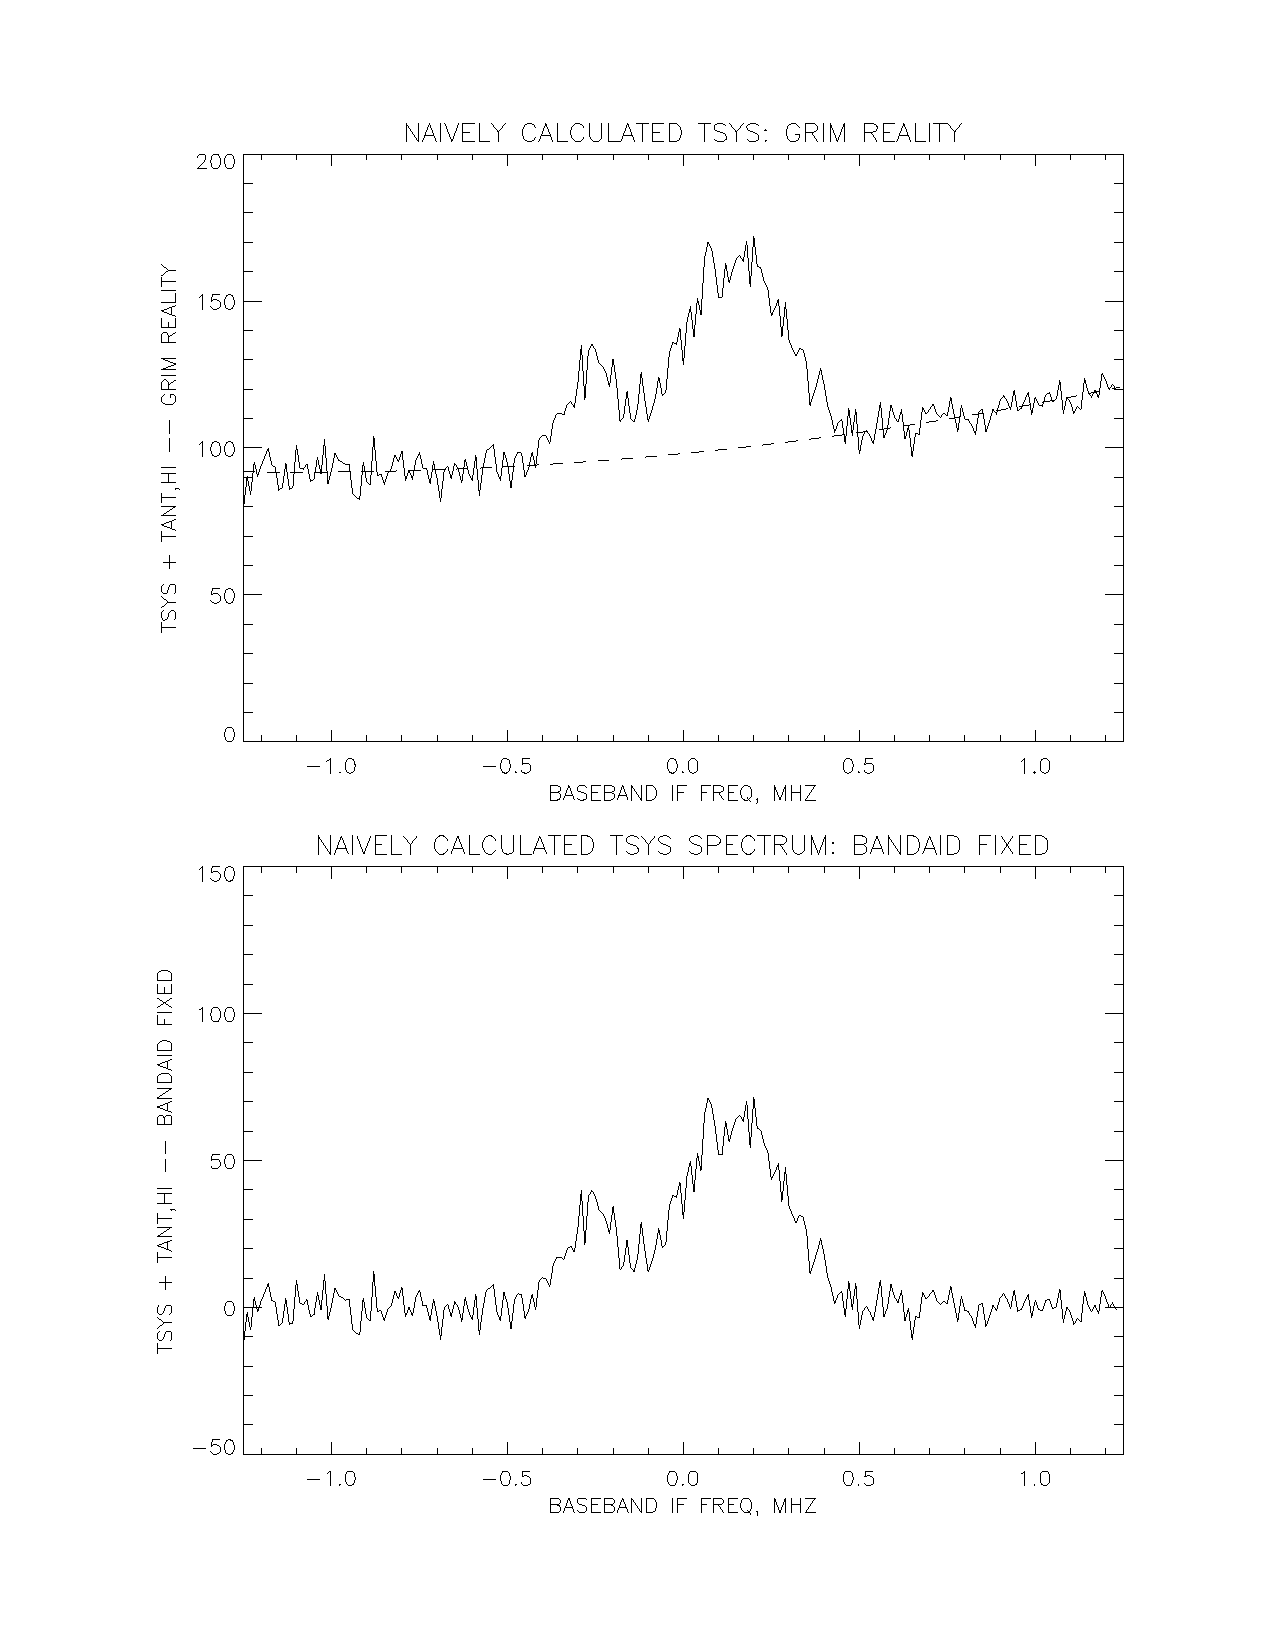
\includegraphics[scale=0.5]{bmp_cal1.pdf}
\end{center}
\vspace{-0.3in}
\caption{\footnotesize A typical raw spectrum with a curvy baseline and
  multiple velocity components. \label{rawspect}}
\end{figure}

Your spectrum will probably look something like that in the top panel of
Figure \ref{rawspect}. There is a zero offset, a curvy baseline, and
one or more spectral peaks. The curvy baseline comes from nonflat
instrumental response, and can be removed with (in order of rigor)
a low-order polynomial fit, an interpolated Fourier fit, or a
covariant eigenmode pseudoinverse, to the 
off-line channels (the approximate
frequency ranges $-1.2 \rightarrow -0.6$ and $ 0.6 \rightarrow 1.2$
MHz).

The dashed line is a second-order polynomial fit to the off-line
channels and the bottom panel has this fit subtracted off.  Here, the
multiple peaks come from HI clouds having different velocities. The
peaks are usually represented as Gaussians with appropriate central
intensities, velocities, and widths.  Fitting Gaussians requires
specifying initial guesses for the component parameters. These guesses
need not be particularly accurate. For example, in the bottom panel of Figure
\ref{rawspect}, initial guesses for the two heights, centers, and widths
(FWHM) could be [20, 50], [-0.3, 0.2] MHz, and [0.01, 0.03] MHz.

After
fitting, check to see if the result looks good: if it does not, then
it's usually because you need one or more additional components. It is
common to require a low-level, broad component that produces no obvious
peak; here, the initial guesses might be [20, 50, 10], [-0.3, 0.2, 0.]
MHz, and [0.01, 0.03, 0.07] MHz. 

These procedures may help you for these least-squares fits, but also
feel free to roll your own data-reduction techniques.
\begin{enumerate}
\item For the polynomial fit, use {\tt numpy.polyfit}

\item For fitting multiple Gaussians, use our home-grown {\tt gaussfit}; for
  evaluating the Gaussians from the parameters produced by {\tt gaussval}, 
  use {\tt gaussval}.
\end{enumerate}

\noindent
In class, we will compare the results from all groups. How reproducible is
our science?

\section {Measuring the Speed of Light in Cables (Group Lab Activity, Week 2)}
\label{expt}

\noindent
For moving power or electronic information from one place to
another, {\it transmission lines} (cables) are
indispensable. It sounds easy---just connect two things with a wire. But
does this really work? We'll explore cables and reflections
by measuring the Voltage Standing Wave Ratio (VSWR), which results from
interference of incident and reflected waves.

The experimental work and measurements described below should
be done by groups.  The analysis in \S \ref{secondweek} should be done
by individuals. The analysis is nontrivial, so don't delay with the
measurements!


\subsection{Estimating Receiver Noise and Gain}

Our receiver system consists of a horn antenna, a pair of amplifiers,
a long length of 50$\Omega$
coaxial cable down from the roof, and then the additional amplifiers and 
filters you see in the rack. In order to obtain a trustworthy calibration,
we must account for the signal loss, gain, and noise
contributions of these various components.

In \S\ref{sec:blackbody} we performed an end-to-end calibration by pointing the antenna into
a known load (you, a $\sim$300 K blackbody). Our goal here is to derive an 
independent cross-check on that calibration by building up 
a model of what is happening to our signal.
To do this, we need to think about the individual components in our system,
as well as the transmission lines that separate them.

Let's start at the end (your SDR) and work backwards.

\subsection{Characterizing the Gain Scale of the SDR}
\label{sec:termination}

As described in class, coaxial cables propagate waves by
providing a uniform (50$\Omega$, ideally frequency-independent) impedance 
along their length, so that each
section of cable receives the outgoing wave from its upstream neighbor
with the same impedance with which it was transmitted. This prevents reflections
from occur along the length of the cable, but they can still arise 
if you do not terminate the cable with the same characteristic impedance.

The end of the line in our receiving system is our SDR module, and we need to
check its input impedance to know how to relate the voltages we measure
to signal power. 
This allows us to calibrate our digitized data.

Inject a signal of known power into the SDR. If you are worried about
cable losses (which are particularly important on long cables), you
might want to use an oscilloscope to measure the signal that your SDR
sees, but beware. The oscilloscope uses 1 M$\Omega$ termination, effectively
acting like you've left the end unconnected. To terminate properly, you will
need to use a T junction to put a $50\Omega$ terminator in parallel with
the oscilloscope.

Next, we need to check the SDR termination to
ensure we are making an apples-to-apples voltage comparison with the
oscilloscope. The easiest way to measure if a cable is properly terminated
is to send a signal in one end and measure if a reflection of that signal
comes back out the same end. Connect
the oscilloscope and a function generator (outputing a square wave) 
to one end of a long cable. For the moment, leave the far end of the cable
unconnected (``floating'').

Zooming in with your oscilloscope, you should be able to see a reflection of the square wave
interfering with the input wave. Notice the time lag between the input and
reflected waves? That tells you about the time it takes to traverse
the cable twice. From that, you can calculate the speed of light
in a cable, which will be helpful later.
Now try terminating the far end of the cable. Did the interference pattern
go away? It should have, because that's the job of termination: to prevent
reflections.

Now repeat this experiment, but with your SDR on the far end
of the cable. Does it properly terminate the cable, or should you
add your own 50$\Omega$ terminator? Does it change if you plug the SDR
in to your RPi? Be aware that termination can change versus frequency,
so you may find that low-frequency signals exhibit a different termination
than high frequencies. How would that affect the waveform you see
on the oscilloscope?

Using everything you know about termination, calculate (with error bars!)
the voltage scale of your SDR, the speed of light on a cable, and the
signal loss per meter through a coaxial BNC cable at 1420 MHz.
In doing your SDR calibration, be sure to keep track of the LO and RF
frequency settings you use, because we also need to calibrate
the spectral response of your SDR relative to this measurement.

\subsubsection{A Note on FIR Filters}

An FIR filter works as an anti-aliasing filter by convolving
28.8 Msps digitized data in the RTL2832U before it is decimated (reduced
in sample rate by throwing out samples) to achieve the sample rate you
specify.
The default coefficients are:
$$
\begin{aligned}
   -54,-36,-41,-40,-32,-14, 14, 53, 101, 156, 215, 273, 327, 372, 404, 421, \\
   421,404,372, 327,273,215,156,101, 53, 14, -14, -32, -40, -41, -36, -54
\end{aligned}
$$ 
(Note the mirror symmetry.) You can change these if you choose.
The 16 numbers you enter are mirrored to generate the full FIR filter.

The Convolution Theorem dicates that the expected (voltage-spectrum)
frequency response is the Fourier transform of these coefficients.
That means you can use {\tt ugradio.dft} to sample the 
filter response at the frequencies
relevant for the Fourier Transforms you will be taking.

With the signal you calibrated and the FIR filter shape you calculated
(or the square of it, for power spectra), you can
partially calibrate an input signal to your SDR module. However, there
appears to be another summing filter in the RTL2832U that is not
well documented. I estimate its coefficients to be something like:
$$
\begin{aligned}
-1/8, -1/4, -3/4, -1/2, -1, 8, -1, -1/2, -3/4, -1/4, -1/8
\end{aligned}
$$
Again, you would use the square of the DFT of these coefficients to correct
the remaining ripple in your power spectrum bandpass shape, after applying
the previous filter correction.

You'll notice my coefficients aren't perfect. Can you do better? Check how
well your coefficients flatten out a white-noise signal.

\subsection{Characterizing Amplifiers, Filters, and Cable Loss}

Following the above steps, we calibrated the input to the SDR, but
that isn't enough to calibrate our telescope the sky signal passes through
amplifiers, filters, and a long cable on the way to our SDR. We need
to calibrate those as well.

Up at the horn, there are 4 amplifiers: three Cougar AC3064C, followed by
one Cougar AC1586C. Look up the gain (in dB) on their respective datasheets
online.

Next, you are going to need to estimate how much signal is lost in the
cable running down from the roof to the 5th floor lab. Fortunately, you
have already characterized the loss in BNC cables per length. Algl you need
to do is figure out how long the cable is, which you can do using the
same square-wave reflectometry you used in \S\ref{sec:termination}.

Finally, you should characterize the gain/loss through the bandpass
filter and mystery ampifiers in the lab. This can be done by injecting a
known signal amplitude and measuring the output with your newly calibrated
SDR module.

\subsection{Antenna Efficiency}

We've characterized the gain in almost every element of our system, except
for one: the antenna. Antennas can be thought of as an impedance-matching
circuit that connects the transmission line of free space (with a characteristic
impedance of 377$\Omega$) to a coaxial transmission line, usually with the
help of an additional balun impedance matching circuit.

In practice, the impedance match of an antenna is imperfect and highly 
frequency-dependent. As a result, not all of an incoming sky signal makes its
way into our receiver; a substantial fraction may reflect and scatter back
out. To account for this, we need an {\bf aperture efficiency}
coefficient that, given the physical area of our antenna's aperture, 
scales how much flux collected over that area actually enters our electronics.
Typical well-matched antennas have efficiencies of 0.6 to 0.7, but poorly matched
antennas can be much lower than this.

For starters, let's assume a well-matched antenna, but be prepared
to revisit this assumption using the results of your end-to-end blackbody load
calibration. If you are clever (and careful), you may also be able to use
the tone injection system to further constrain the aperture efficiency.

If you wish to disconnect or rewire anything at the antenna (to, for example
cross-check the Cougar amplifier gains from the datasheet), you may, but make
sure you leave the system working for the next group.

\section {Statistical Error Analysis (Individually At Home, Week 2)} \label{secondweek}
 
It's time to perform a rigorous, end-to-end calibration of our receiver system,
with the goal of reporting (with correct error bars), the amplitude (in
brightness temperature), Doppler shift (in km/s), and Doppler width (in km/s)
of the spiral arms we observed.

Using your blackbody load calibration and your receiver characterization
to quantify the aperture efficiency of our horn antenna. Estimate the error
in your calibration multiple ways and check for consistency between them.
Estimate the error in your removal of the baseline system temperature.
These are all systematic errors that contribute to our uncertainty.

We also have random (thermal) noise contributing to our uncertainty.
Quantify the noise levels in each individual spectral measurement, per frequency
channel. Ideally, your resultant Gaussian fits should go through your
data points to within the thermal noise. Calculate the reduced chi-square
of your fit. Is it close to one? Can you use $\chi_r$ to argue whether
to use fewer or more Gaussian components in your model?

Finally, estimate the error in your parameter fits using any of the tools
we presented in class. You may do an MCMC fit, per the notebook example,
or quantify a 2-sigma chi-square interval, or use the covariance matrices
of a parameter fitting package. Crucially, include systematic errors on
top of the statistical errors, and make sure, at the end of the day, you believe
your result. Test some numerical simulations to check
your ability to recover true answers.

\end{document}
